% Standalone figure for the Statistical Mechanics notes.
% Build: pdflatex binary-gap.tex  (or run build.sh in this folder)
\documentclass[11pt,tikz,border=2pt]{standalone}
\usepackage{amsmath,amssymb}
\usetikzlibrary{arrows.meta, positioning}
\begin{document}
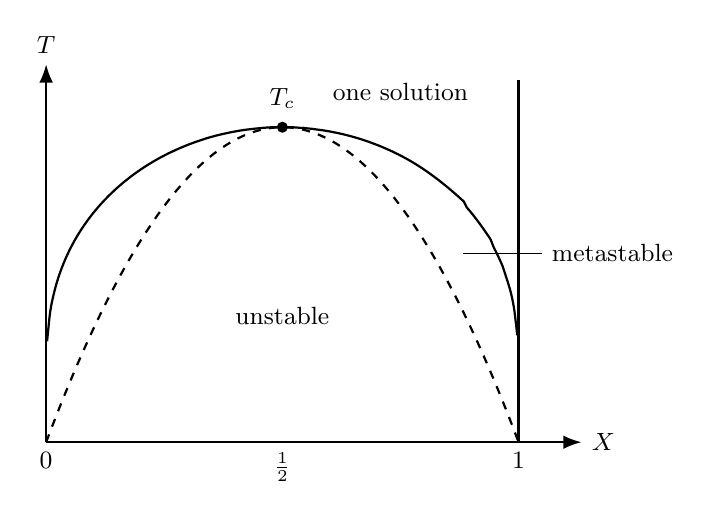
\begin{tikzpicture}[font=\small, >=Latex, line width=0.8pt]
    % axes: x = 6X, y = 4 T/T_c
    \draw[->] (0,0) -- (6.8,0) node[right] {$X$};
    \draw[->] (0,0) -- (0,4.8) node[above] {$T$};
    \draw (6,0) -- (6,4.6);
    \node[below] at (0,0) {$0$};
    \node[below] at (6,0) {$1$};
    \node[below] at (3,0) {$\tfrac12$};
    % binodal T/T_c = 2(1-2X)/ln((1-X)/X)
    \draw[domain=0.002:0.4995, smooth, samples=80, variable=\t]
        plot ({6*\t},{4*2*(1-2*\t)/ln((1-\t)/\t)});
    \draw[domain=0.5005:0.998, smooth, samples=80, variable=\t]
        plot ({6*\t},{4*2*(1-2*\t)/ln((1-\t)/\t)});
    % spinodal T/T_c = 4X(1-X)
    \draw[dashed, domain=0:1, smooth, samples=60, variable=\t]
        plot ({6*\t},{4*4*\t*(1-\t)});
    % critical point
    \fill (3,4) circle (2pt);
    \node[above, yshift=3pt] at (3,4) {$T_c$};
    % labels
    \node at (3,1.6) {unstable};
    \draw[line width=0.4pt] (5.3,2.4) -- (6.3,2.4) node[right] {metastable};
    \node at (4.5,4.45) {one solution};
\end{tikzpicture}
\end{document}
